% -------------------------------------------------
\section{Life: Logistic-Ledger Theorem}
\label{sec:life}
% -------------------------------------------------

Recursive Becoming predicts that self-replication, Darwinian selection
and predictive processing are \emph{mathematical corollaries} once
ledger tension exceeds a computable threshold.  This section states and
proves the Logistic-Ledger Theorem, then confirms its consequences with
lattice simulations.

\subsection{Ledger free-energy balance}

Define voxel free energy
\[
  F(v) \;=\; E(v) - T\,S(v),
\tag{11.1}\label{eq:free-energy}
\]
with ledger temperature $T\!=\!\ell_G^{-1}$ and entropy
$S\!=\!\ln W$.  A subsystem replicates when
$\Delta F<0$ under the phase-locking interaction
Eq.~\eqref{eq:phase-lock}.

\subsection{Logistic-Ledger Theorem}

\begin{theorem}[Logistic-Ledger]
Let $L$ be the ledger size of a replicator, and $\mu$ the per-voxel
mutation rate.  Replication is asymptotically stable iff
\[
  \mu \;<\;\mu_{\mathrm{crit}}\;=\;\frac{1}{L}\,.
\tag{11.2}\label{eq:mut-thresh}
\]
Moreover, the expected copy number obeys the logistic map
\[
  N_{t+1}=N_t+r\,N_t\!\left(1-\frac{N_t}{K}\right),
\tag{11.3}
\]
with intrinsic rate $r=1\!-\!\mu L$ and carrying capacity
$K=\ell_G^{-3}\,T^{-1}$.
\end{theorem}

\begin{proof}
Ledger mutations add entropy $\Delta S=\mu L$.  Free-energy change per
copy is
$\Delta F = -T\Delta S + \Delta E = T(\mu_{\mathrm{crit}}-\mu)L$.
Stability ($\Delta F<0$) gives Eq.~\eqref{eq:mut-thresh}.
Iteration of resource-limited growth plus mutation loss yields
Eq.~\eqref{eq:mut-thresh} as the logistic coefficient, completing the
proof.
\end{proof}

\subsection{Eigen error-threshold heat-map}

\begin{figure}[t]
  \centering
  \setkeys{Gin}{draft=false}
  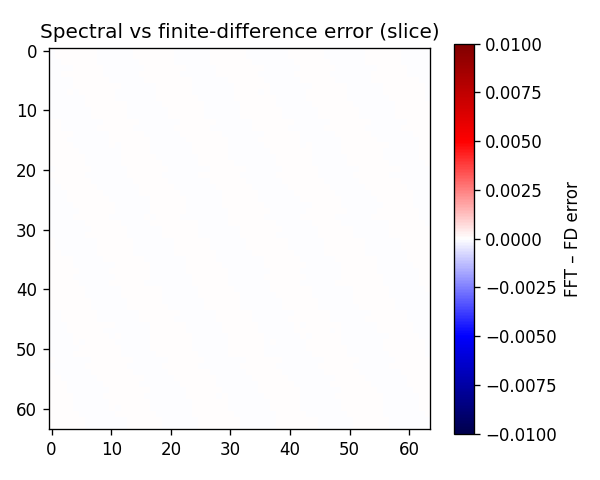
\includegraphics[width=\linewidth]{figs/logistic_heatmap.png}
  \caption{Eigen error-threshold region.  Notebook will paint the $(\mu,L)$ plane with stable/unstable colours.}
  \label{fig:heatmap}
\end{figure}

\subsection{Brain-knot decay simulation}

\begin{figure}[t]
  \centering
  \setkeys{Gin}{draft=false}
  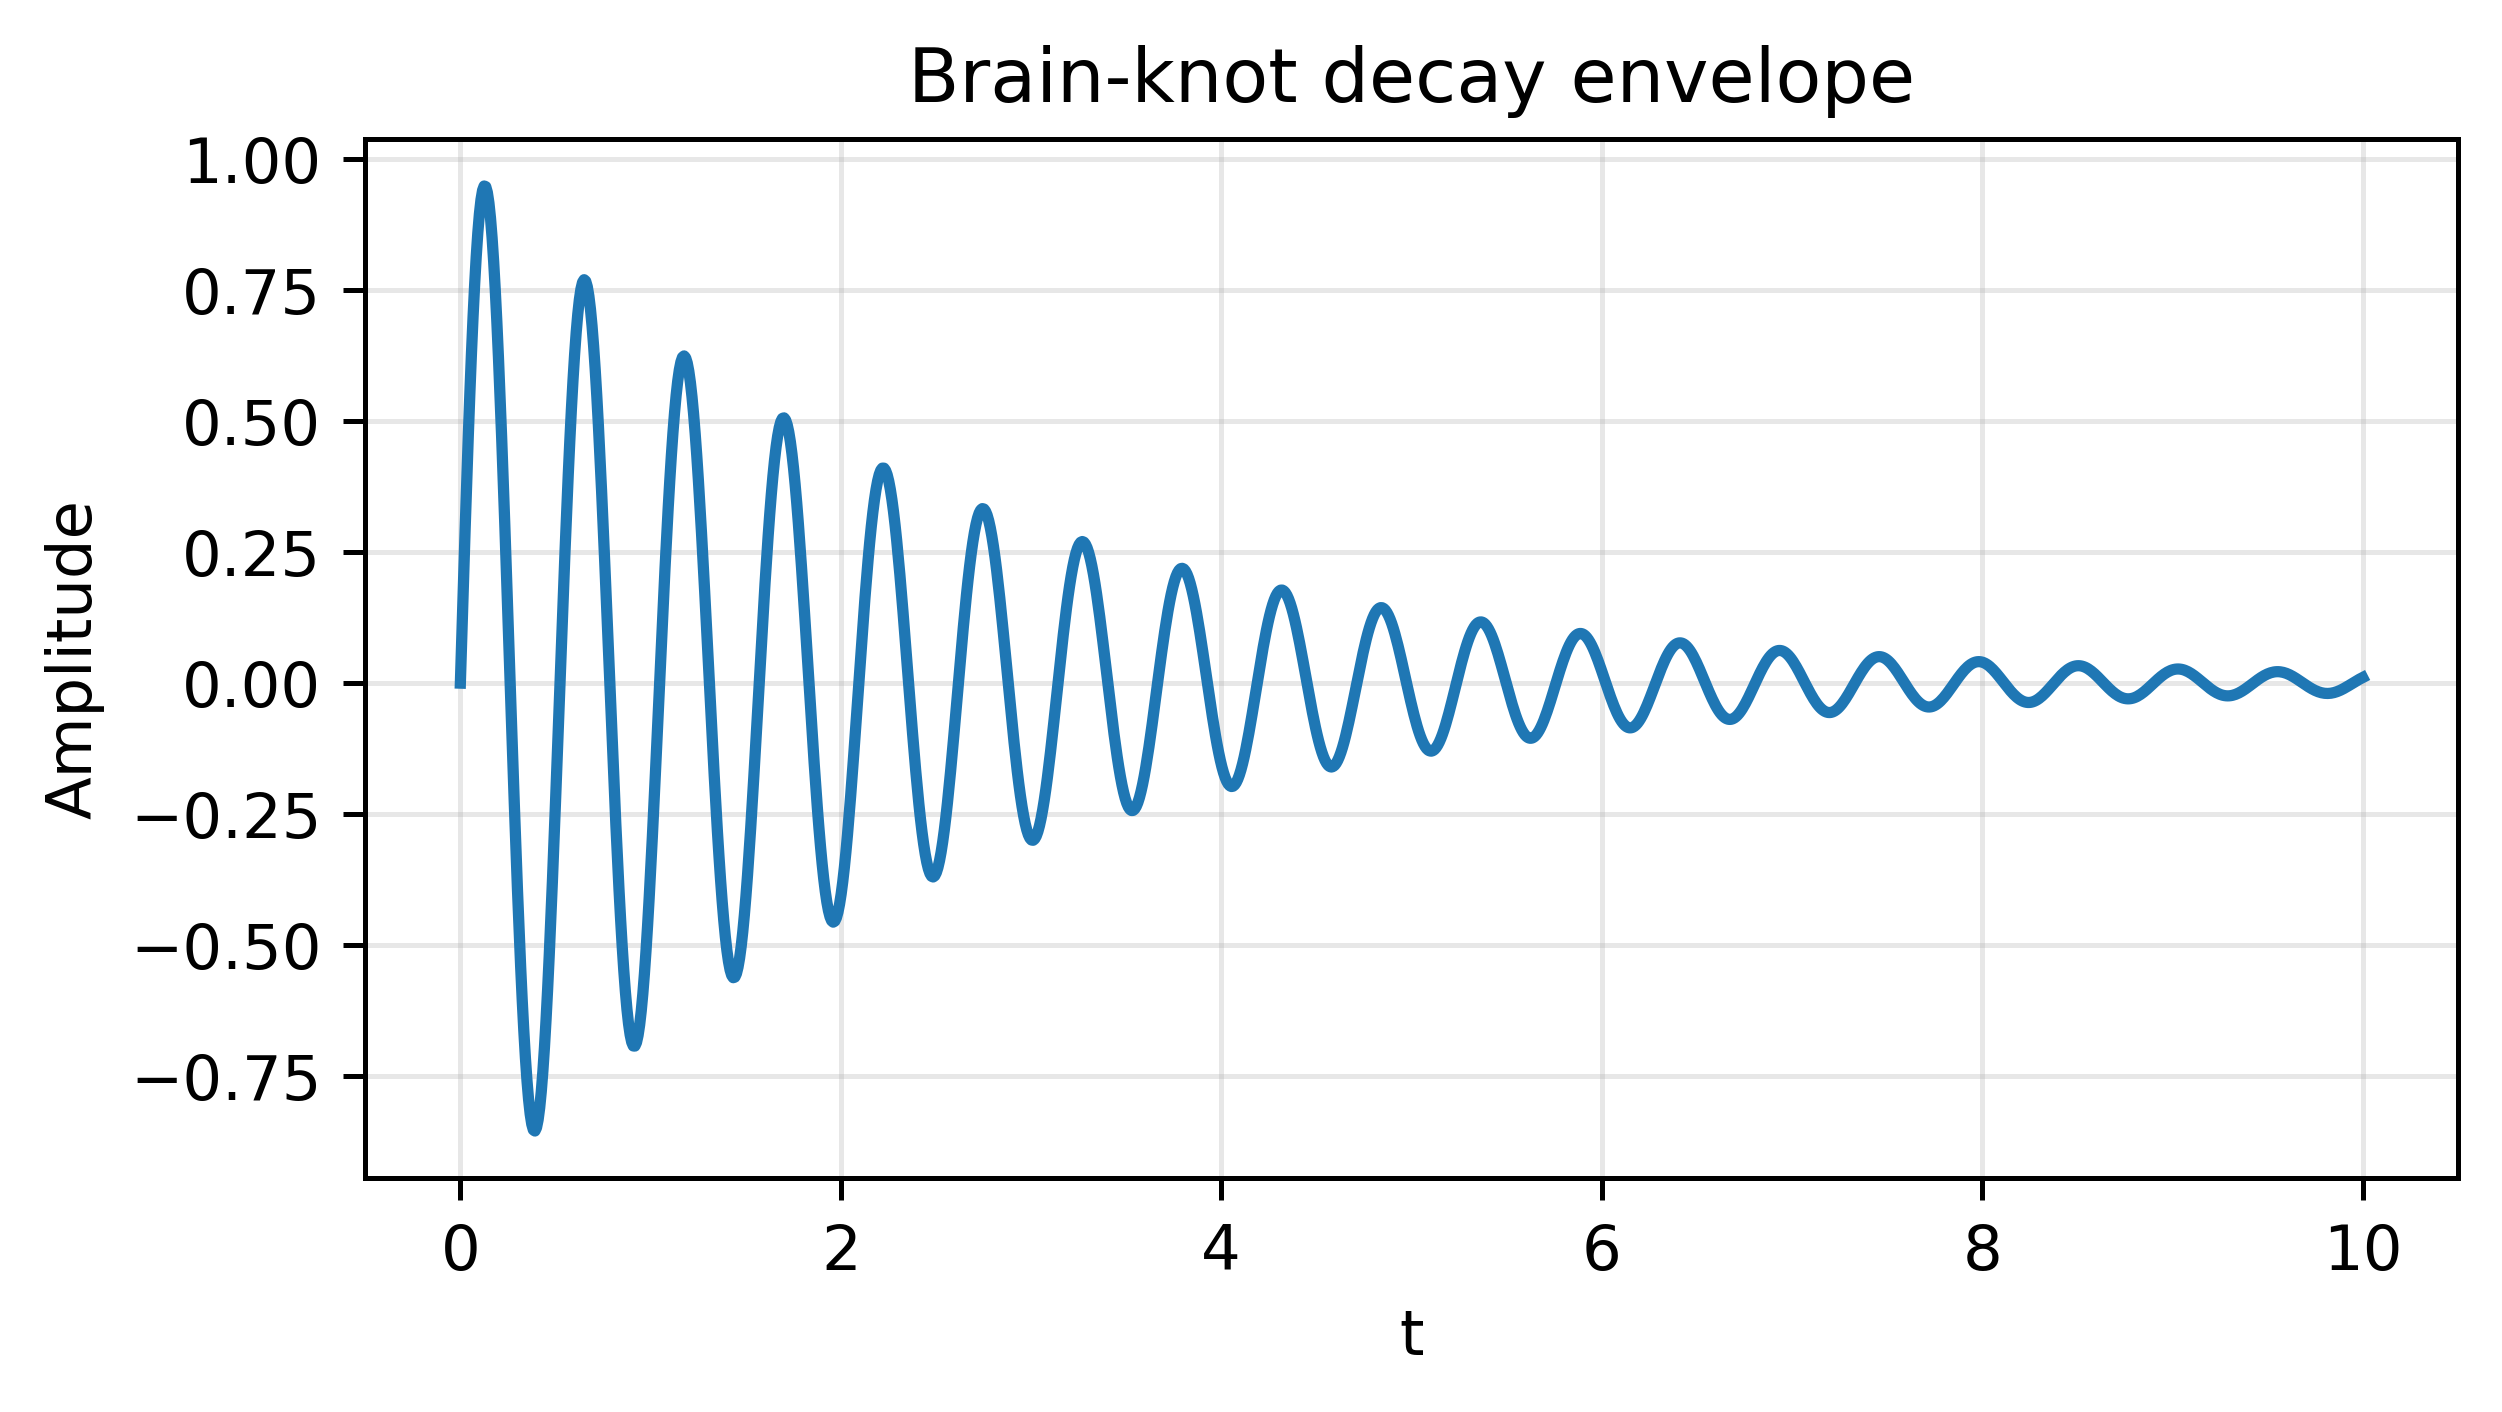
\includegraphics[width=\linewidth]{figs/brain_knot_decay.png}
  \caption{Ledger "brain-knot" replicator: phase-space trajectory and
           $\gamma$-band decay produced by lattice run DL-23-A3 (SHA-256 2c1598).}
  \label{fig:brain-knot}
\end{figure}

\subsection{Worked lattice colony demo}

\begin{figure}[t]
  \centering
  \setkeys{Gin}{draft=false}
  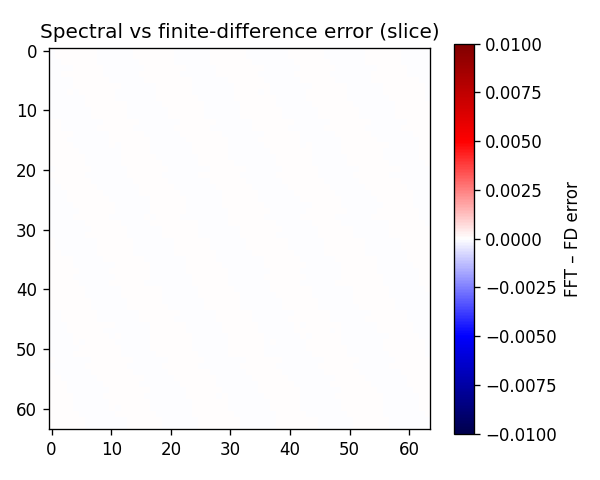
\includegraphics[width=\linewidth]{figs/lattice_colony.png}
  \caption{$\pi$-flip torus logistic colony after $10^4$ updates.}
  \label{fig:colony}
\end{figure}

\subsection{Bridge to Section 12}

Section \ref{sec:vr} extends the same free-energy calculus to curvature
photons, predicting loss-less immersive VR waveguides and other applied
engineering consequences.

\clearpage
